
\chapter{Kombinatorik}

\section{Endliche Summen}
\subsection{Definition}

\begin{Definition}[Summe]\index{Summe}\mbox{}\\*
Für eine Folge $a\colon\Z\to\R$ ist die Summe über die $a_k$
von $k=m$ bis $n$ rekursiv definiert gemäß%
\[
\sum_{k=m}^{m-1} a_k := 0,\qquad
\sum_{k=m}^n a_k := a_n+\sum_{k=m}^{n-1} a_k.
\]
\end{Definition}
Das schaut komplizierter aus als es ist. Man hat
\[\sum_{k=1}^n a_k = a_1+a_2+a_3+\ldots+a_n.\]
Z.\,B. ist
\[\sum_{k=1}^4 k^2 = 1^2+2^2+3^2+4^2 = 1+4+9+16 = 30.\]
Die Berechnung gemäß der Definition:
\begin{align*}
\sum_{k=1}^4 k^2 &= 4^2+\sum_{k=1}^3 k^2
= 4^2+3^2+\sum_{k=1}^2 k^2
= 4^2+3^2+2^2+\sum_{k=1}^1 k^2\\
&= 4^2+3^2+2^2+1^2+\sum_{k=1}^{0} k^2 = 4^2+3^2+2^2+1^2+0 = 30.
\end{align*}

\subsection{Rechenregeln}
\begin{Satz}[Homogenität der Summenoperation]%
\label{Summe-Hom}\index{Homogenität}\mbox{}\\*
Ist $c$ eine Konstante, dann gilt
\[\sum_{k=m}^n ca_k = c\sum_{k=m}^n a_k.\]
\end{Satz}
\strong{Beweis.}
Der Induktionsanfang ist trivial:
\[\sum_{k=m}^{m-1} ca_k = 0 = c\cdot 0 = c\sum_{k=m}^{m-1} a_k.\]
Der Induktionsschritt »$A(n-1)\Rightarrow A(n)$« ist erfüllt, denn es gilt
\[\sum_{k=m}^n ca_k = ca_n+\sum_{k=m}^{n-1} ca_k = ca_n+c\sum_{k=m}^{n-1} a_k
= c\bigg(a_n+\sum_{k=m}^{n-1} a_k\bigg) = c\sum_{k=m}^n a_k.\;\qedsymbol\]

\begin{Satz}[Additivität der Summenoperation]%
\label{Summe-Add}\index{Additivität}\mbox{}\\*
Es gilt
\[\sum_{k=m}^n (a_k+b_k) = \sum_{k=m}^n a_k+\sum_{k=m}^n b_k.\]
\end{Satz}
\strong{Beweis.}
Der Induktionsanfang ist trivial. Induktionsschritt:
\begin{align*}
\sum_{k=m}^n (a_k+b_k) &= (a_n+b_n)+\sum_{k=m}^{n-1} (a_k+b_k)
= (a_n+b_n)+\sum_{k=m}^{n-1} a_k+\sum_{k=m}^{n-1} b_k\\
&= \bigg(a_n+\sum_{k=m}^{n-1}a_k\bigg)+\bigg(b_n+\sum_{k=m}^{n-1}b_k\bigg)
= \sum_{k=m}^n a_k+\sum_{k=m}^n b_k.\;\qedsymbol
\end{align*}

\begin{Satz}[Aufteilung von Summen]%
\label{Summe-Aufteilung}\mbox{}\\*
Für $m\le p\le n$ gilt
\[\sum_{k=m}^n a_k = \sum_{k=m}^{p-1} a_k+\sum_{k=p}^n a_k.\]
\end{Satz}
\strong{Beweis.} Für den Induktionsanfang setzt man $n=p$. Die Gleichung
ist dann erfüllt, weil definitionsgemäß $\sum_{k=p}^p a_k=a_p$
gilt.

Der Induktionsschritt:
\begin{align*}
\sum_{k=m}^n a_k &= a_n+\sum_{k=m}^{n-1} a_k
= a_n + \sum_{k=m}^{p-1} a_k + \sum_{k=p}^{n-1} a_k
= \sum_{k=m}^{p-1} a_k + \sum_{k=p}^n a_k.\;\qedsymbol
\end{align*}

\newpage
\begin{Satz}[Indexshift]%
\label{Summe-Indexshift}\mbox{}\\*
Für die Indexverschiebung der Distanz $d\in\Z$,
kurz Indexshift, gilt%
\[\sum_{k=m}^n a_k = \sum_{k=m+d}^{n+d} a_{k-d}.\]
\end{Satz}
\strong{Beweis.}
Für den Induktionsanfang $n=m-1$ erhält man definitionsgemäß sofort%
\[\sum_{k=m}^{m-1} a_k = 0 = \sum_{k=m+d}^{m+d-1} a_{k-d}.\]
Induktionsschritt:
\begin{align*}
\sum_{k=m}^n a_k = a_n+\sum_{k=m}^{n-1} a_k
= a_{(n+d)-d}+\sum_{k=m+d}^{n+d-1} a_{k-d}
= \sum_{k=m+d}^{n+d} a_{k-d}.\;\qedsymbol
\end{align*}
\strong{Herleitung.} Substituiere $k:=k'-d$. Man formt damit um:%
\begin{align*}
\sum_{k=m}^n a_k = \sum_{m\le k\le n} a_k
= \sum_{m\le k'-d\le n} a_{k'-d}
= \sum_{m+d\le k'\le n+d} a_{k'-d}
= \sum_{k'=m+d}^{n+d} a_{k'-d}.\;\qedsymbol
\end{align*}

\begin{Satz}[Umkehrung der Reihenfolge]%
\label{Summe-Umkehrung}\mbox{}\\*
Es gilt $\sum_{k=0}^n a_k = \sum_{k=0}^n a_{n-k}$.
\end{Satz}
\strong{Beweis.}
Der Induktionsanfang bei $n=0$ ist trivial. Beim Induktionsschritt
macht man sich Satz \ref{Summe-Indexshift} (Indexshift) und
Satz \ref{Summe-Aufteilung} (Aufteilung) zunutze:%
\begin{gather*}
\sum_{k=0}^n a_{n-k} = a_{n-n}+\sum_{k=0}^{n-1} a_{n-k}
= a_0+\sum_{k=0}^{n-1} a_{n-(n-1-k)}
= a_0+\sum_{k=0}^{n-1} a_{k+1}\\
\stackrel{[k:=k-1]}= a_0+\sum_{k=1}^n a_k
= \sum_{k=0}^0 a_k + \sum_{k=1}^n a_k
= \sum_{k=0}^n a_k.\;\qedsymbol
\end{gather*}

\begin{Satz}[Partialsumme der konstanten Folge]%
\label{Summe-der-Eins}\mbox{}\\*
Es gilt
$\sum_{k=m}^n 1 = n-m+1$.
\end{Satz}
\strong{Beweis.} Induktionsanfang bei $n=m-1$:
\[\sum_{k=m}^{m-1} 1=0,\qquad (m-1)-m+1 = m-1-m+1 = 0.\]
Induktionsschritt:
\[\sum_{k=m}^n 1 = 1+\sum_{k=m}^{n-1} 1 = 1+(n-1)-m+1 = n-m+1.\;\qedsymbol\]

\newpage
\begin{Satz}[Partialsumme der arithmetischen Folge]%
\label{Partialsumme-arith}\mbox{}\\*
Es gilt $\sum_{k=0}^n k = \frac{n}{2}(n+1)$.
\end{Satz}
\strong{Beweis.} Der Induktionsanfang $n=0$ ist trivial.
Induktionsschritt:%
\begin{align*}
\sum_{k=0}^n k &= n+\sum_{k=0}^{n-1} k = n+\frac{(n-1)}{2}(n-1+1)
= \frac{2n}{2}+\frac{(n-1)\,n}{2}\\
&= \frac{2n+n^2-n}{2} = \frac{n^2+n}{2}
= \frac{n}{2}(n+1).\;\qedsymbol
\end{align*}
\strong{Herleitung und alternativer Beweis.} Man addiert die Summe
zu sich selbst, da muss das Doppelte der Summe bei herauskommen.
Die Reihenfolge der einen Summe wird mittels Satz \ref{Summe-Umkehrung}
umgekehrt. Danach wendet man Satz \ref{Summe-Add} (Additivität),
Satz \ref{Summe-Hom} (Homogenität) und Satz \ref{Summe-der-Eins} an:%
\begin{align*}
2\sum_{k=0}^n k &= \sum_{k=0}^n k+\sum_{k=0}^n k
= \sum_{k=0}^n k + \sum_{k=0}^n (n-k)\\
&= \sum_{k=0}^n (k+n-k) = \sum_{k=0}^n n
= n\sum_{k=0}^n 1 = n(n+1).\;\qedsymbol
\end{align*}

\begin{Satz}[Partialsumme der geometrischen Folge]\mbox{}\\*
Für $q\ne 1$ gilt $\sum_{k=a}^{b-1} q^k = \frac{q^b-q^a}{q-1}$
\end{Satz}
\strong{Herleitung und Beweis.}
Sei $s:=\sum_{k=a}^{b-1} q^k$ die gesuchte Summe.
Mittels Homogenität und Indexshift findet man
\begin{align*}
qs = q\sum_{k=a}^{b-1} q^k &= \sum_{k=a}^{b-1} q^{k+1} = \sum_{k=a+1}^b q^k = q^b-q^a+\sum_{k=a}^{b-1} q^k
= q^b-q^a+s.
\end{align*}
Das ist nun aber lediglich eine lineare Gleichung in $s$. Die Lösung ist
\[s = \frac{q^b-q^a}{q-1}.\;\qedsymbol\]

\subsection{Anwendungen}

Die gezeigten Rechenregeln ermöglichen die Vereinfachung
einiger Summen, die in der Kombinatorik und Analysis ab
und zu vorkommen. Die allgemeine arithmetischen Folge ist z.\,B.
gegeben gemäß $a_k=Ak+B$, wobei $A,B$ zwei Konstanten sind.
Für die Summe findet man%
\[\sum_{k=0}^n (Ak+B)
= A\sum_{k=0}^n k+B\sum_{k=0}^n 1 = A\,\frac{n}{2}(n+1)+B(n+1)
= \Big(\frac{An}{2}+B\Big)(n+1),\]
bzw.
\[\sum_{k=1}^n (Ak+B)
= A\sum_{k=1}^n k + B\sum_{k=1}^n 1
= A\,\frac{n}{2}(n+1)+Bn = \Big(\frac{A}{2}(n+1)+B\Big)n.\]

\newpage
\subsection{Teleskopsummen}

\begin{Satz}[Teleskopsumme]\mbox{}\\*
Es gilt $\sum_{k=m}^{n-1} (a_{k+1}-a_k) = a_n-a_m$.
\end{Satz}
\strong{Beweis.}
Mittels Indexshift stellt man die folgende Überlegung an:
\begin{gather*}
\sum_{k=m}^{n-1} a_{k+1}
= \sum_{k=m+1}^n a_k = a_n-a_m+\sum_{k=m}^{n-1} a_k.
\end{gather*}
Benutzung dieser Überlegung führt zu:
\begin{gather*}
\sum_{k=m}^{n-1} (a_{k+1}-a_k)
= \sum_{k=m}^{n-1} a_{k+1}-\sum_{k=m}^{n-1} a_k
= a_n-a_m+\sum_{k=m}^{n-1} a_k-\sum_{k=m}^{n-1} a_k
= a_n-a_m.\;\qedsymbol
\end{gather*}

\begin{Definition}[Differenzoperator]\mbox{}\\*
Für eine Folge $(a_n)$ definiert man
$(\Delta a)_n := a_{n+1}-a_n.$
\end{Definition}
Die Teleskopsumme lässt sich damit in der Form
$\sum_{k=m}^{n-1}(\Delta a)_k = a_n-a_m$
schreiben. Der Leser wird jetzt vielleicht fragen, warum für diesen
einfachen Zusammenhang explizit ein Operator definiert wurde.
Nun ja, dieser Operator kann iteriert werden. Die Formeln die
dabei herauskommen, sind nicht mehr ganz so einfach. Z.\,B. ist
\begin{align*}
(\Delta^2 a)_n &= (\Delta \Delta a)_n
= (\Delta a)_{n+1}-(\Delta a)_n
= (a_{n+2}-a_{n+1}) - (a_{n+1}-a_n)\\
&= a_{n+2}-2a_{n+1}+a_n.
\end{align*}
Außerdem genügt der Differenzoperator selbst bestimmten Rechenregeln.
\begin{Satz}
Der Operator $\Delta$ ist linear, d.\,h. für
Folgen $(a_n)$, $(b_n)$ und eine Konstante $c$ gilt%
\[\Delta(c\cdot a) = c\cdot\Delta a,\qquad
\Delta(a+b) = (\Delta a)+(\Delta b).\]
\end{Satz}
\strong{Beweis.} Man findent
\begin{gather*}
\Delta (ca)_n = ca_{n+1}-ca_n
= c(a_{n+1}-a_n) = c\Delta a_n
\end{gather*}
und
\begin{align*}
\Delta (a+b)_n &= (a_{n+1}+b_{n+1})-(a_n+b_n)
= a_{n+1}-a_n + b_{n+1}-b_n\\
&= (\Delta a)_n + (\Delta b)_n.\;\qedsymbol
\end{align*}
Der Differenzoperator erlaubt es, nach vielen neuen Summenformeln
zu fischen, nämlich indem man einen beliebigen Ausdruck nimmt und
diesen als Teleskopsumme darstellt. Für $a_n=n^2$ ist z.\,B.
\[(\Delta a)_n = (n+1)^2-n^2 = n^2+2n+1-n^2 = 2n+1.\]
Damit bekommt man
\begin{gather*}
2\sum_{k=0}^{n-1} k + n = \sum_{k=0}^{n-1} (2k+1) = 
\sum_{k=0}^{n-1} (\Delta a)_k
= n^2-0^2 = n^2.
\end{gather*}
Umformung bringt
\[\sum_{k=0}^{n-1} k = \frac{1}{2}(n^2-n) = \frac{n}{2}(n-1).\]
Setzt man für $n$ nun $n+1$ ein, dann ergibt sich die schon
bekannte Formel von Satz \ref{Partialsumme-arith}.

Eine wichtige Formel für Teleskopsummen gilt
bezüglich Def. \ref{def:ffac}.

\begin{Satz}\label{diff-ffac}
Sei $k\ge 0$. Für $a_n:=n^{\underline k}$ gilt
$(\Delta a)_n = kn^{\underline{k-1}}$.
\end{Satz}
\strong{Beweis.} Der Fall $k=0$ ist trivial. Für $k\ge 1$
wendet man Satz \ref{ffac-n-rec} an:
\begin{gather*}
(\Delta a)_n = (n+1)^{\underline k}-n^{\underline k}
= (n-(k-1)+1)(n+1)^{\underline {k-1}}-(n+1-k)n^{\underline{k-1}}\\
= (n+1)n^{\underline{k-1}}-(n+1-k)n^{\underline{k-1}}
= (n+1-n-1+k)n^{\underline{k-1}} = kn^{\underline{k-1}}.\;\qedsymbol
\end{gather*}
Für $a_n:=\tfrac{k^{\underline {p+1}}}{p+1}$ ergibt sich
demnach $(\Delta a_n) = k^{\underline p}$. Das führt zur
Teleskopsumme
\[\sum_{k=m}^{n-1} k^{\underline p}
= \frac{n^{\underline{p+1}}-m^{\underline{p+1}}}{p+1}.\]
Nun treten zumeist Summen über $k^p$ auf und nicht
über $k^{\underline p}$. Zwischen diesen gibt es aber einen
einfachen Zusammenhang. Nämlich lässt sich $x^n$ als
Linearkombination
\[x^n = \sum_{k=0}^n S_k x^{\underline k}\]
darstellen. Die Linearfaktoren $S_k$ sind von besonderer
Bedeutung, es sind die Stirling"=Zahlen zweiter Art.
\begin{Definition}[Stirling-Zahlen zweiter Art]\mbox{}\\*
Man definiert rekursiv
\[n>0\implies\begin{Bmatrix}n\\ k\end{Bmatrix} :=
k\begin{Bmatrix}n-1\\ k\end{Bmatrix}
+\begin{Bmatrix}n-1\\ k-1\end{Bmatrix},\]
mit den Anfangswerten
\[\begin{Bmatrix}n\\ n\end{Bmatrix} := 1,\qquad
k=0<n\lor n<k\implies\begin{Bmatrix}n\\ k\end{Bmatrix} := 0.\]
\end{Definition}
\begin{Satz}\label{power-stirling}
Für $x\in\R$ und $n\in\N_0$ gilt
\[x^n = \sum_{k=0}^n \begin{Bmatrix}n\\ k\end{Bmatrix} x^{\underline k}.\]
\end{Satz}
Unter Anwendung von Satz \ref{power-stirling}
und der Teleskopsumme zu Satz \ref{diff-ffac} gelangt man zu
\begin{gather*}
\sum_{k=m}^{n-1} k^p = \sum_{k=m}^{n-1} \sum_{i=0}^p
\begin{Bmatrix}p\\ i\end{Bmatrix}k^{\underline i}
= \sum_{i=0}^p \begin{Bmatrix}p\\ i\end{Bmatrix}\sum_{k=m}^{n-1}
k^{\underline i}
= \sum_{i=0}^p \begin{Bmatrix}p\\ i\end{Bmatrix}
\frac{n^{\underline{i+1}}-m^{\underline{i+1}}}{i+1}.
\end{gather*}
Hiermit lassen ich alle Potenzsummen vereinfachen. Der Leser
rechne zur Übung die folgenden Resultate nach:
\begin{align}
\sum_{k=0}^n k^2 &= \tfrac{1}{3}n^3+\tfrac{1}{2}n^2+\tfrac{1}{6}n
= \tfrac{n}{6}(n+1)(2n+1),\\
\sum_{k=0}^n k^3 &= \tfrac{1}{4}n^4+\tfrac{1}{2}n^3+\tfrac{1}{4}n^2
= (\tfrac{n}{2}(n+1))^2.
\end{align}

\subsection{Ungleichung zwischen Summen}

\begin{Korollar}
Für zwei Folgen $(a_k)$, $(b_k)$ gilt
\[(\forall k\ge m)(a_k\le b_k)\implies\sum_{k=m}^n a_k \le \sum_{k=m}^n b_k.\]
\end{Korollar}
\strong{Beweis.} Induktiv. Induktionsanfang ist $0\le 0$ wegen $\sum_{k=m}^{m-1} x_k=0$.
Gemäß \eqref{lele-add} gilt
\[\sum_{k=m}^{n-1} a_k\le\sum_{k=m}^{n-1} b_k
\implies \underbrace{a_n+\sum_{k=m}^{n-1} a_k}_{\sum_{k=m}^n a_k}
\le \underbrace{b_n+\sum_{k=m}^{n-1} b_k}_{_{\sum_{k=m}^n b_k}}.\;\qedsymbol\]


\newpage
\section{Endliche Produkte}

\subsection{Definition}
\begin{Definition}[Produkt]\mbox{}\\*
Für eine Folge $a\colon\Z\to\R$ ist das Produkt der $a_k$ für
$k$ von $k=m$ bis $k=n$ rekursiv definiert gemäß%
\[\prod_{k=m}^{m-1} a_k := 1,\qquad
\prod_{k=m}^n a_k := a_n\cdot\prod_{k=m}^{n-1} a_k.\]
\end{Definition}

\subsection{Rechenregeln}
Für Produkte gelten analoge Rechenregeln wie für Summen. Auch
die Beweise sind analog, weshalb sie für den Leser als Übung
dienen sollen.%
\begin{Satz}
Ist $c\in\R$ eine Konstante, dann gilt%
\[\prod_{k=m}^n ca_k = c^n\prod_{k=m}^n a_k.\]
\end{Satz}
\begin{Satz}
Es gilt
\[\prod_{k=m}^n a_k b_k = \prod_{k=m}^n a_k \prod_{k=m}^n b_k.\]
\end{Satz}
\begin{Satz}[Aufteilung von Produkten]\label{Prod-Aufteilung}
Für $m\le p\le n$ gilt:
\[\prod_{k=m}^n a_k = \prod_{k=m}^{p-1} a_k\prod_{k=p}^n a_k.\]
\end{Satz}
\begin{Satz}[Indexshift]\label{Prod-Indexshift}
Für die Indexverschiebung der Distanz $d\in\Z$ gilt%
\[\prod_{k=m}^n a_k = \prod_{k=m+d}^{n+d} a_{k-d}.\]
\end{Satz}

\newpage
\section{Potenzen}

\begin{Definition}
Sei $(M,\cdot,e)$ ein Monoid. Für $a\in M$ und $n\in\N_0$ ist die
$n$-te Potenz von $a$ rekursiv definiert gemäß
\[a^0 := e, \quad a^n = a\cdot a^{n-1}.\]
\end{Definition}
\begin{Satz}
Es gilt $a^n = \prod_{k=1}^n a$.
\end{Satz}
\strong{Beweis.} Induktionsanfang: $a^0=e=\prod_{k=1}^0 a$.
Induktionsschritt:
\[a^n = a\cdot a^{n-1} = a\cdot\prod_{k=1}^{n-1} a
= \prod_{k=1}^n a.\;\qedsymbol\]

\begin{Satz}
Es gilt $a^{m+n}=a^m a^n$.
\end{Satz}
\strong{Beweis.} Induktionsanfang:
$a^{0+n} = a^n = ea^n = a^0 a^n$.
Induktionsschritt:
\[a^{m+n} = a^{(m-1)+n+1} = aa^{(m-1)+n} = aa^{m-1}a^n
= a^m a^n.\;\qedsymbol\]

\begin{Satz}
Unter der Voraussetzung $ab=ba$ gilt $(ab)^n = a^n b^n$.
\end{Satz}
\strong{Beweis.} Induktionsanfang: $(ab)^0 = e = ee = a^0 b^0$.
Induktionsschritt:
\[(ab)^n = (ab)(ab)^{n-1} = aba^{n-1}b^{n-1}
= aa^{n-1}bb^{n-1} = a^n b^n.\]
Achtung, wir müssen noch $ab^n = b^na$ aufzeigen.

Induktionsanfang: $ab^0 = ae = a = ea = b^0a$.

Induktionsschritt:
$ab^n = abb^{n-1} = bab^{n-1} = bb^{n-1}a = b^na$.\;\qedsymbol

\newpage
\section{Permutationen und Variationen}%
\index{Permutation}

\subsection{Anzahl der Permutationen}

Gegeben sind zwei unterschiedliche Buchstaben, sagen wir $A,B$. Diese
Buchstaben sind auf zwei Plätze zu legen, wobei die Reihenfolge die
wesentliche Rolle spielt. Wie viele Möglichkeiten gibt es dafür?
Das sind zwei, nämlich $AB$ und $BA$. Man sagt, es gibt zwei
Permutationen der Buchstaben $A,B$.

Wie viele Möglichkeiten gibt es, die drei Buchstaben $A,B,C$ auf
drei Plätze zu legen? Es sind sechs, das sind
$ABC$, $BAC$, $ACB$, $BCA$, $CAB$ und $CBA$. Man sagt, es gibt
sechs Permutationen der Buchstaben $A,B,C$.

Das ist schon recht unübersichtlich. Es gibt aber eine systematische
Methode, alle Möglichkeiten aufzuzählen. Für den ersten Platz gibt
es drei Möglichkeiten. Für den zweiten Platz gibt es dann jeweils
nur noch zwei Möglichkeiten, weil nur noch zwei Buchstaben zur
Verfügung stehen. Für den letzten Platz bleibt jeweils eine
Möglichkeit. Somit ergibt sich die folgende Baumstruktur:

\begin{figure}[h]
\begin{center}
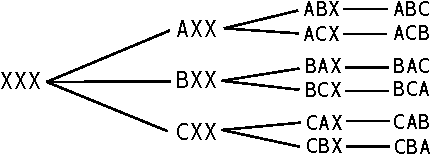
\includegraphics[width=0.5\textwidth]{img/Perm-ABC.pdf}
\end{center}
\end{figure}

\noindent
Gegeben sind nun $n$ Buchstaben und genau so viele freie Plätze.
Die Anzahl der Permutationen nennen wir $n!$, sprich \emph{$n$ Fakultät}.
Für den ersten Platz gibt es $n$ Möglichkeiten. Für den zweiten Platz
sind nur noch jeweils $n-1$ Buchstaben übrig, es gibt deshalb nur noch
jeweils $n-1$ Möglichkeiten. Für den dritten Platz gibt es noch jeweils
$n-2$ Möglichkeiten, für den vierten Platz jeweils $n-3$ usw. Für den
$n$-ten Platz gibt es schließlich jeweils nur noch eine Möglichkeit.
Das macht insgesamt%
\[n! = n\cdot (n-1)\cdot (n-2)\cdot\ldots\cdot 3\cdot 2\cdot 1\]
Möglichkeiten. Außerdem ergibt sich die folgende Rekursionsformel:%
\[n! = n\cdot (n-1)!.\]
\begin{Definition}[Fakultät]%
\index{Fakultaet@Fakultät}\label{def:fac}\mbox{}\\*
Für eine Zahl $n\in\N_0$ ist die Fakultät von $n$ rekursiv
definiert gemäß%
\[0! := 1,\qquad n! := n\cdot (n-1)!.\]
\end{Definition}
Wir zuvor gezeigt, gibt es genau $n!$ Permutationen von $n$
unterschiedlichen Objekten. Es gibt $4!=24$ Permutationen
der vier Buchstaben $A,B,C,D$, aber schon $5!=120$ Permutationen der
fünf Buchstaben $A,B,C,D,E$. Die Anzahl der Permutationen wächst
rasant. Es gibt z.\,B. unzählige Möglichkeiten, Bücher in ein
längeres Buchregel zu stellen.


\subsection{Anzahl der Variationen ohne Wiederholung}%
\index{Variationen!ohne Wiederholung}

Angenommen man hat wieder $n$ unterschiedliche Buchstaben
zur Verfügung, aber nur noch $k$ freie Plätze, wobei $k\le n$.
Wie bei den Permutationen ergeben sich für den ersten Platz
$n$ Möglichkeiten, für den zweiten jeweils noch $n-1$,
für den dritten jeweils noch $n-2$ usw. Im Gegensatz zum
Baum der Permutationen bricht der Baum nun vorläufig
nach dem $k$-ten Platz ab. Die Anzahl der Möglichkeiten schreiben
wir $n^{\underline k}$ und sprechen von der absteigenden Faktoriellen
von $n$ mit $k$ Faktoren. Man erhält%
\[n^{\underline k} = \prod_{i=0}^{k-1} (n-i)
= n\cdot (n-1)\cdot (n-2)\cdot\ldots\cdot (n-k+1).\]
Offenbar gilt $n^{\underline n} = n!$, das ist der Spezialfall $k=n$.

Das Produkt haben wir ja rekursiv definiert. Durch Einsetzen dieser
Definition lässt sich daraus die rekursive Definition der absteigenden
Faktoriellen extrahieren:

\begin{Definition}[Absteigende Faktorielle]\index{Faktorielle}%
\index{absteigende Faktorielle}\index{fallende Faktorielle}%
\label{def:ffac}\mbox{}\\*
Die absteigende Faktorielle von $n$ mit $k$ Faktoren ist rekursiv
definiert gemäß%
\[n^{\underline 0} := 1,\qquad
n^{\underline k} := (n-k+1)\,n^{\underline{k-1}}.\]
\end{Definition}

\begin{Satz}\label{ffac-fac}
Für $n,k\in\N_0$ und $k\le n$ gilt
\[n^{\underline k} = \frac{n!}{(n-k)!}.\]
\end{Satz}
\strong{Beweis.} Kann man ohne langes Überlegen induktiv
machen.

Induktionsanfang:
\[n^{\underline 0} = 1,\qquad \frac{n!}{(n-0)!}=\frac{n!}{n!}=1.\]

Induktionsschritt »$A(k-1)\Rightarrow A(k)$«:
\begin{align*}
n^{\underline k} &= (n-k+1)\,n^{\underline{k-1}}
= (n-k+1)\frac{n!}{(n-(k-1))!}
= (n-k+1)\frac{n!}{(n-k+1)!}\\
&= (n-k+1)\frac{n!}{(n-k+1)(n-k)!}
= \frac{n!}{(n-k)!}.\;\qedsymbol
\end{align*}

\noindent
Hierbei wurde $(n-k+1)!=(n-k+1)(n-k)!$ benutzt, was gemäß
der rekursiven Definition der Fakultät gilt.

\strong{Alternativer Beweis.} Mittels Satz \ref{Prod-Aufteilung}
(Produktaufteilung) und  Satz \ref{Prod-Indexshift} (Indexshift):%
\begin{align*}
n! &= \prod_{i=0}^{n-1}(n-i)
= \prod_{i=0}^{k-1} (n-i) \prod_{i=k}^{n-1} (n-i)
= n^{\underline k} \prod_{i=k}^{n-1} (n-i)\\
&\stackrel{[i:=i+k]}= n^{\underline k}\prod_{i=0}^{n-k-1} (n-k-i)
= n^{\underline k}\,(n-k)!.\;\qedsymbol
\end{align*}

\begin{Satz}\label{ffac-n-rec}
Für $n,k\in\Z$ und $k\ge 0$ gilt
\[(n-k+1)(n+1)^{\underline k} = (n+1)n^{\underline k}.\]
\end{Satz}
\strong{Beweis.} Für $k\ge 1$ gilt
\[(n-k+1)\prod_{i=0}^{k-2}(n-1)
= (n-(k-1))\prod_{i=0}^{k-2} (n-i) = \prod_{i=0}^{k-1}(n-i).\]
Damit ergibt sich
\begin{gather*}
(n-k+1)(n+1)^{\underline k} = (n-k+1)\prod_{i=0}^{k-1} (n+1-i)
= (n-k+1)(n+1)\prod_{i=1}^{k-1}(n+1-i)\\
= (n+1)(n-k+1)\prod_{i=0}^{k-2}(n-i)
= (n+1)\prod_{i=0}^{k-1}(n-i)
= (n+1)n^{\underline k}.
\end{gather*}
Den Fall $k=0$ verifiziert man separat:
\[(n-0+1)(n+1)^{\underline 0}
= (n-0+1)\cdot 1 = (n+1)\cdot 1 = (n+1)n^{\underline 0}.\;\qedsymbol\]

% \newpage
\subsection{Anzahl der Variationen mit Wiederholung}%
\index{Variationen!mit Wiederholung}

Lässt man die Möglichkeit zu, einen schon gelegten Buchstaben
nochmals zu legen, dann ergeben sich offenbar mehr Möglichkeiten.
Wie viele Möglichkeiten gibt es, die zwei Buchstaben $A,B$
auf drei freie Plätze zu legen? Dazu ergibt sich der folgende
Baum:

\begin{figure}[h]
\begin{center}
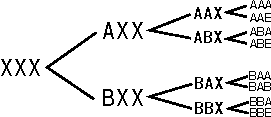
\includegraphics[width=0.38\textwidth]{img/VariW-XXX-AB.pdf}
\end{center}
\end{figure}

\noindent
Offenbar darf jeder Platz unabhängig von den anderen mit $A$ oder
$B$ belegt werden. Das macht zwei Möglichkeiten für den ersten
Platz, dann jeweils zwei Möglichkeiten für den zweiten Platz,
und dann jeweils zwei Möglichkeiten für den dritten Platz.
Insgesamt sind es%
\[8 = 2^3 = 2\cdot 2\cdot 2\]
Möglichkeiten.

Allgemein hat man nun $n$ unterschiedliche Buchstaben und $k$
freie Plätze. Nach der gleichen Argumentation wie zuvor muss die
Anzahl der Möglichkeiten%
\[n^k = \underbrace{n\cdot n\cdot n\cdot\ldots\cdot n}_\text{$k$ Faktoren}\]
sein.

Z.\,B. kann man sich die Frage stellen, wie viele unterschiedliche
Werte ein Byte annehmen kann. Ein Byte besitzt acht Bits, also $k=8$,
und jedes dieser Bits kann unabhängig von den anderen entweder 0 oder 1
sein, d.\,h. $n=2$. Das macht $2^8=256$ Werte.

\subsection{Deutung als Anzahl der Abbildungen}

Betrachten wir nochmals die Variationen mit Wiederholung. Jedoch werden
die Buchstaben nun nicht auf die Plätze gelegt, sondern den Plätzen
werden Buchstaben zugeordnet. Das läuft natürlich aufs Selbe hinaus,
bloß dass es aus der anderen Richtung betrachtet wird. Jeder Platz
erhält eine Nummer, angefangen mit null. Jeder nummerierte Platz
bekommt einen Buchstaben, das ist aber nichts anderes als eine
Abbildung. Für zwei Buchstaben $A,B$ und drei freie Plätze
erhält man
\[f\colon X\to Y,\quad X:=\{0,1,2\},\quad Y:=\{A,B\}.\]
Die Anzahl der Variationen mit Wiederholung ist genau die Anzahl
der unterschiedlichen möglichen Abbildungen. Nennen wir die Menge aller
Abbildungen $\Abb(X,Y)$, dann ist nach $|{\Abb(X,Y)}|$ gefragt.
Wie schon bekannt ist, gilt%
\[|{\Abb(X,Y)}| = |Y|^{|X|}.\]
Bei den Variationen ohne Wiederholung müssen alle Buchstaben
unterschiedlich sein. Unter der neuen Sichtweise bedeutet das aber
nichts anderes, als dass die Abbildung eine injektive sein muss.
Nennt man die Menge aller Injektionen $\operatorname{Inj}(X,Y)$,
dann gilt wie bereits gezeigt%
\[|{\operatorname{Inj}(X,Y)}| = |Y|^{\underline{|X|}}.\]
Die Permutationen sind ein Spezialfall der Variationen,
wo $|X|=|Y|$ ist. Weil die Injektion endlich ist, und es genau
so viele Elemente im Definitionsbereich wie in der Zielmenge gibt,
muss die Injektion auch surjektiv sein. Die Menge aller Bijektionen
nennen wir $\operatorname{Bij}(X,Y)$. Man kann jetzt auch einfach
die Buchstaben so nummerieren wie die Plätze, dann ist $X=Y$,
man erhält eine Selbstabbildung. Wie schon bekannt, ergibt sich%
\[|{\operatorname{Bij}(X,X)}| = |{\operatorname{Inj}(X,X)}|
= |X|^{\underline{|X|}} = |X|!.\]


